% Created 2026-07-01 Wed 22:46
% Intended LaTeX compiler: pdflatex
\documentclass[table, aspectratio=169]{beamer}
\usepackage[utf8]{inputenc}
\usepackage[T1]{fontenc}
\usepackage{graphicx}
\usepackage{longtable}
\usepackage{wrapfig}
\usepackage{rotating}
\usepackage[normalem]{ulem}
\usepackage{amsmath}
\usepackage{amssymb}
\usepackage{capt-of}
\usepackage{hyperref}
\usepackage[T1]{fontenc}
\usepackage[utf8]{inputenc}
\usepackage[spanish]{babel}
\usepackage[backend=biber, style=apa]{biblatex}
\addbibresource{/home/stevenech/S9-Memoria-del-Sistema/bibliography/bibliography.bib}
\usepackage[default]{sourcesanspro}
\usetheme{metropolis}
\setbeamertemplate{navigation symbols}{}
\setbeamersize{text margin left=2.5em, text margin right=2.5em}
\usepackage{tcolorbox}
\usepackage{colortbl}
\usepackage{tikz}
\usetikzlibrary{positioning,arrows.meta,calc}
\usepackage{booktabs}
\usepackage{array}
\definecolor{BgDark}{HTML}{0D1E30}
\definecolor{GoldTitle}{HTML}{F0C040}
\definecolor{LightBlue}{HTML}{7ECFFF}
\definecolor{MintGreen}{HTML}{A8E6CF}
\definecolor{HitGreen}{HTML}{00B894}
\definecolor{MissRed}{HTML}{D63031}
\definecolor{WarnColor}{HTML}{FF7675}
\definecolor{TableHeadBg}{HTML}{1E3A5A}
\definecolor{TableBodyBg}{HTML}{141E2C}
\definecolor{TableBorder}{HTML}{2A4A6A}
\definecolor{PyReg}{HTML}{c0392b}
\definecolor{PyL1}{HTML}{d35400}
\definecolor{PyL2}{HTML}{f1c40f}
\definecolor{PyRam}{HTML}{2ecc71}
\definecolor{PySSD}{HTML}{2980b9}
\definecolor{PyDisk}{HTML}{8e44ad}
\setbeamercolor{background canvas}{bg=BgDark}
\setbeamercolor{normal text}{fg=white}
\setbeamercolor{palette primary}{bg=TableHeadBg, fg=LightBlue}
\setbeamercolor{frametitle}{bg=TableHeadBg, fg=LightBlue}
\setbeamercolor{title}{fg=GoldTitle}
\setbeamercolor{subtitle}{fg=MintGreen}
\setbeamercolor{progress bar}{fg=HitGreen, bg=LightBlue!30}
\setbeamercolor{title separator}{fg=GoldTitle}
\setbeamercolor{alerted text}{fg=WarnColor}
\setbeamercolor{itemize item}{fg=GoldTitle}
\setbeamercolor{block title}{bg=TableHeadBg, fg=GoldTitle}
\setbeamercolor{block body}{bg=BgDark!80!white, fg=white}
\setbeamercolor{section in toc}{fg=GoldTitle}
\setbeamercolor{subsection in toc}{fg=LightBlue}
\tcbset{caja base/.style={boxrule=0pt, leftrule=5pt, sharp corners=west, arc=8pt, fontupper=\small, boxsep=2pt, left=6pt, right=6pt, top=4pt, bottom=4pt, before skip=0.5em, after skip=0.5em}}
\newtcolorbox{conceptobox}[1][]{caja base, colback=LightBlue!15!BgDark, colframe=LightBlue, title={#1}, coltitle=BgDark, fonttitle=\bfseries}
\newtcolorbox{conceptotemporal}[1][]{caja base, colback=GoldTitle!15!BgDark, colframe=GoldTitle, title={#1}, coltitle=BgDark, fonttitle=\bfseries}
\newtcolorbox{conceptoespacial}[1][]{caja base, colback=MintGreen!15!BgDark, colframe=MintGreen, title={#1}, coltitle=BgDark, fonttitle=\bfseries}
\newtcolorbox{conceptowarn}[1][]{caja base, colback=WarnColor!15!BgDark, colframe=WarnColor, title={#1}, coltitle=white, fonttitle=\bfseries}
\newtcolorbox{conceptohit}[1][]{caja base, colback=HitGreen!15!BgDark, colframe=HitGreen, title={#1}, coltitle=BgDark, fonttitle=\bfseries}
\newtcolorbox{cajaimagen}[1][]{boxrule=1.5pt, arc=6pt, colback=white, colframe=LightBlue, boxsep=2pt, left=2pt, right=2pt, top=2pt, bottom=2pt, halign=center}
\newcommand{\verde}[1]{\textcolor{HitGreen}{\textbf{#1}}}
\newcommand{\rojo}[1]{\textcolor{MissRed}{\textbf{#1}}}
\newcommand{\highlight}[1]{\textcolor{GoldTitle}{\textbf{#1}}}
\usetheme{metropolis}
\author{Lenin G. Falconí}
\date{}
\title{S9 — Memoria del Sistema}
\hypersetup{
 pdfauthor={Lenin G. Falconí},
 pdftitle={S9 — Memoria del Sistema},
 pdfkeywords={},
 pdfsubject={},
 pdfcreator={Emacs 27.1 (Org mode 9.3)}, 
 pdflang={Spanish}}
\begin{document}

\maketitle

\section{Indicaciones}
\label{sec:org8a8f8af}
\begin{frame}[label={sec:org40ff79e}]{Reparto y Bibliografía}
\begin{itemize}
\item Reparto del tema por grupos:
\begin{itemize}
\item \alert{G3:} Estructura del sistema de Memoria + Memoria Caché.
\item \alert{G4:} Memoria Interna (DRAM, SRAM, ROM), Corrección de Errores (Hamming), Organización Avanzada.
\end{itemize}
\item Fuentes bibliográficas:
\begin{itemize}
\item \textcite{stallings2006esp}, 7ma edición, 2006, Capítulos 5 y 6.
\item \textcite{stallings2022computer}, 11ava edición, 2022, Capítulos 4, 5 y 6.
\end{itemize}
\end{itemize}
\end{frame}

\section{Estructura del sistema de Memoria}
\label{sec:org97dfd22}
\begin{frame}[label={sec:orgab37af6}]{Jerarquía de Memoria}
\begin{center}
\begin{tikzpicture}[node distance=2mm,
    every node/.style={draw=none,minimum height=0.8cm,font=\small\bfseries,align=center,text=white,rounded corners=3pt}]
  \node[fill=PyReg,text width=3cm]            (reg)  {Registros};
  \node[fill=PyL1,text width=4.5cm,below=2mm of reg]   (cac)  {Caché (\textbf{SRAM})};
  \node[fill=PyRam,text width=6cm,below=2mm of cac]     (ram)  {Memoria Principal (\textbf{DRAM})};
  \node[fill=PySSD,text width=6cm,below=2mm of ram]     (rom)  {Firmware (\textbf{ROM})};
  \node[fill=PyDisk,text width=7.5cm,below=2mm of rom]   (disk) {Almacenamiento Secundario};
\end{tikzpicture}
\end{center}
\vspace{2mm}
\begin{center}\scriptsize\textcolor{LightBlue}{
  Hacia abajo: $\uparrow$ capacidad, $\downarrow$ costo/bit \quad\vline\quad
  Hacia arriba: $\uparrow$ velocidad}
\end{center}
\end{frame}

\section{Memoria Interna}
\label{sec:org3533016}
\begin{frame}[label={sec:orgb086438}]{DRAM y SRAM: Principios Básicos}
\begin{columns}[T]
  \begin{column}{0.48\textwidth}
    \begin{conceptobox}[DRAM (RAM Dinámica)]
      El estándar para Memoria Principal.
    \end{conceptobox}x
    \begin{itemize}
      \item \textbf{Estructura:} 1 transistor + 1 condensador.
      \item \textbf{Lógica:} El bit se almacena como \textit{carga eléctrica} (naturaleza analógica).
      \item \textbf{Reto:} El condensador pierde carga rápidamente. Requiere un \textcolor{WarnColor}{\textbf{refresco periódico}} para no perder los datos.
    \end{itemize}
  \end{column}
  
  \begin{column}{0.48\textwidth}
    \begin{conceptotemporal}[SRAM (RAM Estática)]
      El estándar para Memoria Caché.
    \end{conceptotemporal}
    \begin{itemize}
      \item \textbf{Estructura:} 6 transistores configurados como un biestable (Flip-Flop).
      \item \textbf{Lógica:} Dispositivo puramente digital.
      \item \textbf{Ventaja:} Mientras haya energía, el dato es estable. \textcolor{HitGreen}{\textbf{No necesita refrescos}}.
    \end{itemize}
  \end{column}
\end{columns}
\end{frame}

\begin{frame}[label={sec:org53adbde}]{DRAM vs SRAM: La gran decisión}
¿Por qué no usar la memoria más rápida en todo el sistema? La respuesta está en la física:

\vspace{4mm}
\begin{table}
\centering\large
\setlength{\tabcolsep}{18pt}
\renewcommand{\arraystretch}{1.5}
\begin{tabular}{@{}lcc@{}}
  \rowcolor{TableHeadBg}
   & \textcolor{LightBlue}{\textbf{DRAM (Dinámica)}} & \textcolor{LightBlue}{\textbf{SRAM (Estática)}} \\
  \rowcolor{TableBodyBg}
  \textbf{Densidad (Costo)} & \verde{Muy Alta (Barata)} & \rojo{Baja (Costosa)} \\
  \rowcolor{TableBodyBg}
  \textbf{Velocidad}        & \rojo{Lenta} & \verde{Muy Rápida} \\
  \rowcolor{TableBodyBg}
  \textbf{Refresco}         & \rojo{Sí (Consume ciclos)} & \verde{No (Constante)} \\
  \rowcolor{TableBodyBg}
  \textbf{Uso Ideal}        & Memoria Principal (RAM) & Memoria Caché (L1/L2) \\
\end{tabular}
\end{table}
\end{frame}

\begin{frame}[label={sec:org29fd52c}]{Evolución de las Memorias ROM}
\begin{conceptobox}[La necesidad de flexibilidad]
  La ROM nació como "Solo Lectura", pero la necesidad de actualizar el firmware impulsó métodos de borrado cada vez más avanzados.
\end{conceptobox}
\vspace{2mm}

\begin{itemize}[<+->]
  \item \highlight{ROM (Máscara):} Programada físicamente en fábrica. \rojo{Imborrable} y cero margen de error.
  \item \highlight{PROM:} Programable por el usuario \textit{una sola vez} (quemando fusibles internos).
  \item \highlight{EPROM:} Borrable con \azul{luz ultravioleta} (tarda hasta 20 minutos y borra \textit{todo} el chip).
  \item \highlight{EEPROM:} Borrable \azul{eléctricamente a nivel de byte}. Flexible, pero costosa y menos densa.
  \item \highlight{Flash Memory:} Borrable eléctricamente \verde{por bloques}. Combina la altísima densidad de EPROM con la flexibilidad eléctrica. ¡El estándar actual!
\end{itemize}
\end{frame}

\section{Corrección de Errores}
\label{sec:orgd1d05d9}
\begin{frame}[label={sec:org03341c2}]{Control de Errores en Memoria}
Para lidiar con los errores, se implementan lógicas de detección y corrección en el flujo de lectura y escritura de la memoria.

\vspace{4mm}
\begin{center}
  \begin{cajaimagen}
    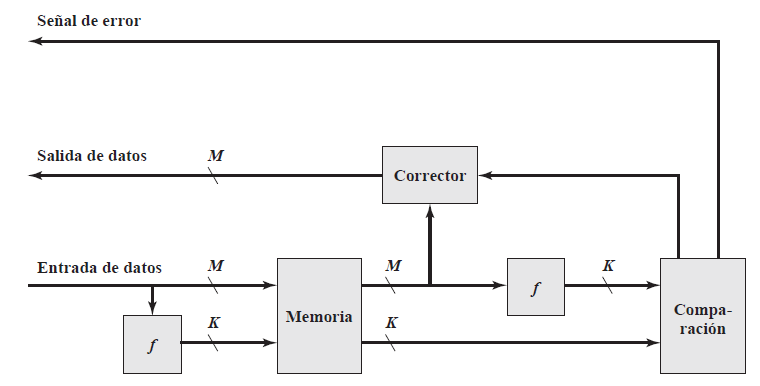
\includegraphics[width=0.8\textwidth, keepaspectratio]{imagenes/Figura_5_7.png}
  \end{cajaimagen}
\end{center}
\end{frame}

\begin{frame}[label={sec:org0aafa3f}]{Hard Error vs Soft Error}
Los sistemas de memoria están sujetos a fallos. Se dividen en dos familias principales:

\vspace{3mm}

\begin{conceptowarn}[Hard Error (Fallo Físico)]
  Un defecto \textbf{permanente} en el hardware. Celdas fundidas que se quedan atascadas en 0 o 1. \\
  $\rightarrow$ \textbf{Causas:} Desgaste, defectos de fábrica. \\
  $\rightarrow$ \textbf{Solución:} \rojo{Irreversible}. Hay que reemplazar el chip.
\end{conceptowarn}

\vspace{2mm}

\begin{conceptohit}[Soft Error (Fallo Transitorio)]
  Un evento \textbf{aleatorio y no destructivo}. Un bit "voltea" de 0 a 1 por accidente, pero el chip está sano. \\
  $\rightarrow$ \textbf{Causas:} Ruido eléctrico, \highlight{radiación natural} (partículas alfa). \\
  $\rightarrow$ \textbf{Solución:} \verde{Corregible}. Si lo detectamos, podemos volver a escribir el bit correcto.
\end{conceptohit}
\end{frame}

\begin{frame}[label={sec:orgfc130c4}]{Código de Hamming: Concepto General}
Para corregir un \textit{Soft Error}, no basta con saber \textit{que} ocurrió un error, tenemos que saber \textbf{exactamente dónde ocurrió}.
\begin{columns}[c]
  \begin{column}{0.5\textwidth}
    \begin{itemize}
      \item \textbf{La idea:} Añadir bits redundantes (paridad) a nuestros datos.
      \item Richard Hamming descubrió que ubicando estos guardianes en posiciones que son \highlight{potencias de 2}, podemos generar un código matemático infalible.
      \item El cruce de información (intersección en los diagramas de Venn) delata matemáticamente al bit dañado.
    \end{itemize}
  \end{column}
  \begin{column}{0.5\textwidth}
    \begin{cajaimagen}
      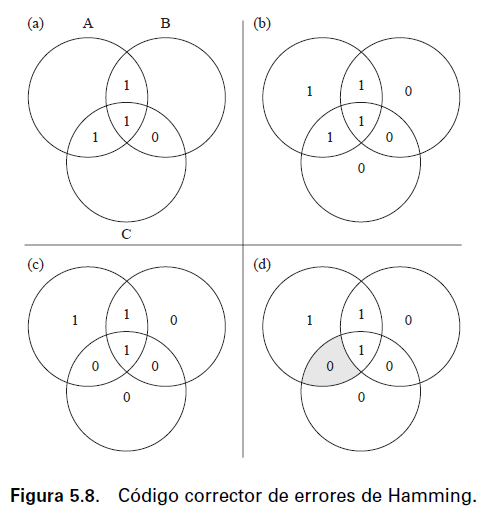
\includegraphics[width=0.85\textwidth, keepaspectratio]{imagenes/Figura_5_8.png}
    \end{cajaimagen}
  \end{column}
\end{columns}
\end{frame}

\begin{frame}[label={sec:org18bb0d5}]{Código de Hamming: Generación (Paso 1)}
\textbf{1. Datos a enviar (4 bits):} \texttt{1011} (D1, D2, D3, D4) \\
\textbf{2. Posiciones:} Metemos los datos dejando libres las potencias de 2 (P1, P2, P4).

\begin{center}
\begin{tikzpicture}[every node/.style={draw=none,minimum size=0.75cm,font=\scriptsize\bfseries, text=white, rounded corners=2pt}]
  \foreach \i/\lab/\col in {1/P1/PyL1, 2/P2/PyL1, 3/1/PySSD, 4/P4/PyL1, 5/0/PySSD, 6/1/PySSD, 7/1/PySSD}{
    \node[fill=\col] (p\i) at (\i*0.85,0) {\lab};
    \node[draw=none,font=\tiny, text=white!70] at (\i*0.85,0.55) {\i};
  }
\end{tikzpicture}
\end{center}

\vspace{2mm}
\textbf{3. Cálculo de la Paridad} (Las zonas vigiladas deben sumar una cantidad par de '1's):
\begin{itemize}
  \item \textbf{P1} vigila saltando de 1 en 1 (pos 1, 3, 5, 7): $P1 \oplus 1 \oplus 0 \oplus 1 = 0 \implies \highlight{P1 = 0}$
  \item \textbf{P2} vigila saltando de 2 en 2 (pos 2, 3, 6, 7): $P2 \oplus 1 \oplus 1 \oplus 1 = 0 \implies \highlight{P2 = 1}$
  \item \textbf{P4} vigila saltando de 4 en 4 (pos 4, 5, 6, 7): $P4 \oplus 0 \oplus 1 \oplus 1 = 0 \implies \highlight{P4 = 0}$
\end{itemize}

\vspace{2mm}
\textbf{Mensaje final transmitido hacia la memoria:}
\begin{center}
\begin{tikzpicture}[every node/.style={draw=none,minimum size=0.75cm,font=\scriptsize\bfseries, text=white, rounded corners=2pt}]
  \foreach \i/\val/\col in {1/0/PyL1, 2/1/PyL1, 3/1/PySSD, 4/0/PyL1, 5/0/PySSD, 6/1/PySSD, 7/1/PySSD}{
    \node[fill=\col] (p\i) at (\i*0.85,0) {\val};
  }
\end{tikzpicture}
\end{center}
\end{frame}

\begin{frame}[label={sec:orgf86d39e}]{Código de Hamming: Error y Corrección (Paso 2)}
\begin{conceptowarn}[¡Impacto de partícula radiactiva!]
  El bit en la \textbf{posición 6} cambia de \texttt{1} a \texttt{0} de forma silenciosa.
\end{conceptowarn}

\textbf{Palabra dañada leída por el procesador:}
\begin{center}
\begin{tikzpicture}[every node/.style={draw=none,minimum size=0.75cm,font=\scriptsize\bfseries, text=white, rounded corners=2pt}]
  \foreach \i/\val/\col in {1/0/PyL1, 2/1/PyL1, 3/1/PySSD, 4/0/PyL1, 5/0/PySSD, 6/0/MissRed, 7/1/PySSD}{
    \node[fill=\col] (p\i) at (\i*0.85,0) {\val};
    \node[draw=none,font=\tiny, text=white!70] at (\i*0.85,0.55) {\i};
  }
\end{tikzpicture}
\end{center}

\textbf{4. Detección (Síndrome):} El hardware recalcula las sumas de paridad.
\begin{itemize}
  \item \textbf{S1} (pos 1, 3, 5, 7): $0 \oplus 1 \oplus 0 \oplus 1 = \rojo{0}$ (¡Todo bien!)
  \item \textbf{S2} (pos 2, 3, 6, 7): $1 \oplus 1 \oplus \rojo{0} \oplus 1 = \verde{1}$ (¡Hay un error!)
  \item \textbf{S4} (pos 4, 5, 6, 7): $0 \oplus 0 \oplus \rojo{0} \oplus 1 = \verde{1}$ (¡Hay un error!)
\end{itemize}

\begin{conceptohit}[La magia matemática]
  Tomamos los valores de error y armamos el Síndrome binario (S4 S2 S1) = $110_2 = \highlight{6}$. \\
  ¡El hardware detecta instantáneamente que el bit 6 falló y lo invierte, recuperando el dato!
\end{conceptohit}
\end{frame}

\section{Organización Avanzada de Memorias RAM}
\label{sec:org117df01}
\begin{frame}[label={sec:org137b322}]{DDR SDRAM y Memorias Flash (11, 216)}
\begin{itemize}
\item Desarrollo del resto del tema por parte del grupo de exposición.
\end{itemize}

\printbibliography
\end{frame}
\end{document}
